\documentclass{article}

\usepackage{polski}
\usepackage[polish]{babel}
\usepackage[utf8]{inputenc}
\usepackage[T1]{fontenc}
\usepackage{graphicx}
\usepackage{float}

\title{Agate Evolver}
\author{Wojciech Ciszewski \and Alicja Dutkiewicz \and Stanisław Kurdziałek \\[1cm]{Opiekun: Piotr Szymczak}}
\date{19.02.2019}

\begin{document}
\maketitle
\section{Wstęp}
Niniejszy projekt powstał w ramach Hackathonu 2.0 Wydziału Fizyki UW. Jego celem jest przetestowanie prostego modelu powstawania agatów poprzez zasymulowanie w oparciu o niego powstawania kolejnych warstw minerału.

Końcowym efektem naszej pracy jest \textit{Agate evolver}, który produkuje strukturę warstw dla danej początkowej geometrii agatu w dwóch i, w niektórych przypadkach, trzech wymiarach. Przetestowaliśmy go na rzeczywistych agatach, aby sprawdzić, czy numerycznie wygenerowana struktura pasm pokrywa się z rzeczywistą.


\section{Opis modelu}
Agaty to minerały złożone z mikrokrystalicznej krzemionki ułożonej w charakterystyczne warstwy. Agaty wypełniają zwykle pustki po pęcherzach gazowych uwięzionych w stygnącej lawie. Jedna z teorii ich powstawania mówi, że kolejne warstwy krzemionki osadzały się na ściankach takiej pustki, a kolorowe paski są odzwierciedleniem różnych w składzie chemicznym roztworu na przestrzeni setek tysięcy lat, w czasie których tworzył się agat.

Szukaliśmy kształtów poszczególnych warstw agatu zakładając, że wzrost (w kierunku od ścianek do środka buły agatowej) odbywa się ze stałą prędkością (czyli nowa warstwa składa się z punktów będących w ustalonej odległości od warstwy poprzedniej). Taki wzrost ma naturalną tendencję do generowania „ostrych kantów”. Takie punkty z nieciągłą pochodną są często widoczne w agatach, co jest argumentem za tym, że ten prosty model wzrostu może być w tym przypadku właściwy.

\subsection{Model 2D}
W modelu 2D traktowaliśmy kolejne warstwy jako płaskie krzywe zamknięte, którą można przybliżyć wielokątami. Wykorzystaliśmy klasy \texttt{Polygon}\\
i \texttt{MultiPolygon} z modułu \texttt{geometry} biblioteki \texttt{shapely}.

Stworzyliśmy funkcję \texttt{evolve\_agat} pozwalającą wygenerować przekrój agatu o zadanym konturze. Funkcja przyjmuje następujące argumenty:
\begin{description}
\item[\texttt{first\_layer}] \hfill \\
lista wierzchołków zewnętrznej warstwy \texttt{[(x1, y1), (x2, y2), ... ]}
\item[\texttt{layer\_width}] \hfill \\
odległość pomiędzy kolejnymi warstwami. Domyślnie \texttt{0.05}
\item[\texttt{min\_area}] \hfill \\
powierzchnia wnętrza agatu. Domyślnie \texttt{0.001}
\item[\texttt{N\_apexes}] \hfill \\
maksymalna liczba wierzchołków wielokątów reprezentujących kolejne wartswy. Jeśli równa \texttt{-1} (domyślnie), to tyle samo co w \texttt{first\_layer}
\item[\texttt{fig}] \hfill \\
obiekt klasy \texttt{Figure} z biblioteki \texttt{matplotlib}, na którym ma zostać narysowany wynik symulacji. Domyślnie przyjmuje wartość \texttt{None} i rysunek jest wyświetlany po wywołaniu funkcji
\end{description}

Ewolucję schematycznie przedstawia rysunek \ref{ewolucja_2d}. W każdym kroku ewolucji za pomocą metody \texttt{buffer} znajdowany był zbiór $N=\texttt{N\_apexes}$ punktów odległych o \texttt{layer\_width} od aktualnej warstwy ($[(x_1,y_1), (x_2, y_2), ..., (x_N, y_N)]$) i znajdujących się wewnątrz wielokąta --- te punkty tworzyły kolejną warstwę ($[(x_1',y_1'), (x_2', y_2'), ..., (x_N', y_N')]$). Jej wnętrze $A$ kolorowano na jeden z losowo wybranych kolorów. Następnie przypisywano $x_i \leftarrow x_i'$, $y_i \leftarrow y_i'$ i rozpoczynał się kolejny krok. Ewolucję kontynuowano, aż powierzchnia wielokąta $A$ reprezentującego aktualną warstwę była mniejsza niż \texttt{min\_area}.
\begin{figure}[H]
\caption{Ilustracja kroku ewolucji 2D}
\label{ewolucja_2d}
\centering
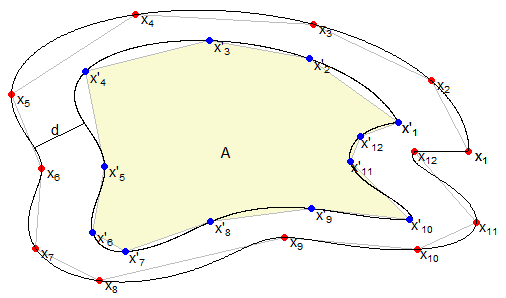
\includegraphics[width=0.7\textwidth]{obrazy/ewolucja2d.png}
\end{figure}
\subsubsection{Generowanie konturów}
Sztuczne agaty generowaliśmy za pomocą funkcji $r(\varphi)=\frac{1}{1+\alpha} (1 + \frac{\alpha}{1+\alpha}\sin(\beta\varphi)^2)$. Przykłady można zobaczyć na rysunkach \ref{wygenerowany1}, \ref{wygenerowany2} i \ref{wygenerowany3}.
\begin{figure}[H]
\caption{\texttt{evolve\_agat(polar\_curve(modulation = 0.3, freq = 2/3))}}
\label{wygenerowany1}
\centering
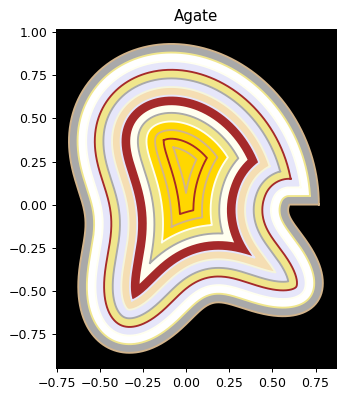
\includegraphics[width=0.5\textwidth]{obrazy/wygenerowany1.png}
\end{figure}
\begin{figure}[H]
\caption{\texttt{evolve\_agat(polar\_curve(modulation = 0.5, freq = 2/3))}}
\label{wygenerowany2}
\centering
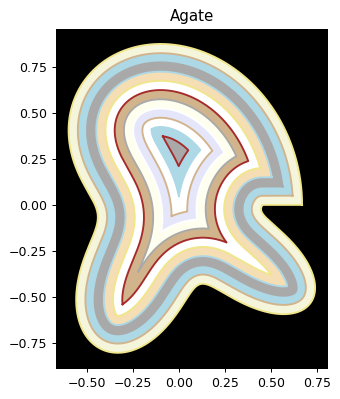
\includegraphics[width=0.5\textwidth]{obrazy/wygenerowany2.png}
\end{figure}
\begin{figure}[H]
\caption{\texttt{evolve\_agat(polar\_curve(modulation = 0.3, freq = 1))}}
\label{wygenerowany3}
\centering
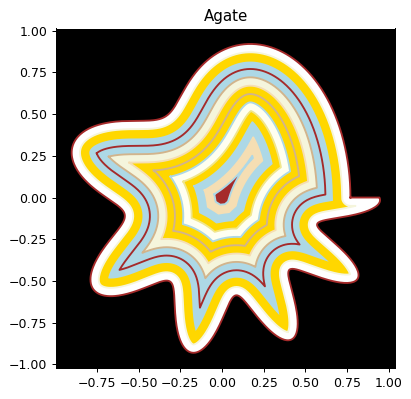
\includegraphics[width=0.5\textwidth]{obrazy/wygenerowany3.png}
\end{figure}
\subsection{Model 3D}
Rzeczywiste agaty należy traktować jak trójwymiarowe bryły --- ewolucja dwuwymiarowych warstw odpowiada rzeczywistej jedynie w przypadku, gdy agat jest wystarczająco długi, a jego przekrój poprzeczny --- wolno zmienny. Rozważmy dowolną zamkniętą, dwuwymiarową powierzchnię wypukłą $\Gamma$. W przybliżeniu możemy taką powierzchnię traktować jak zbiór dwuwymiarowych zamkniętych konturów będących kolejnymi przekrojami poprzecznymi danej powierzchni oddalonymi od siebie o pewną stałą odległość $d$. Przekroje takie można z kolei przybliżać wielokątami, jak w przypadku $2D$. Pojedyncza warstwa trójwymiarowego agatu jest więc przechowywana w pamięci programu jako lista obiektów klasy \texttt{MultiPolygon}. Dodatkowo przechowywana jest odległość $d$ między kolejnymi przekrojami poprzecznymi.

Funkcję generującą kolejną warstwę trójwymiarowego agatu stworzyliśmy w oparciu o dwuwymiarową wersję. Kluczowym było spostrzeżenie, że obszar o jaki urośnie dany przekrój poprzeczny jest sumą wkładów od jego własnego przyrostu i przyrostu sąsiednich przekrojów. Niech $l$ będzie odległością o jaką narasta warstwa w pojedynczym kroku (\texttt{layer\_width} w programie). Załóżmy, że w pamięci przechowywanych jest $n$ przekrojów każdej warstwy numerowanych liczbami całkowitymi $0,1,2,...,n-1$. Aby znaleźć kolejną warstwę należy znaleźć jej wszystkie przekroje. Wkład przekroju o numerze $k$ danej warstwy do przekroju o tym samym numerze kolejnej wartwy wyznaczamy używając stosownej funkcji dla przypadku dwuwymiarowego. Wkład przekroju o numerze $k$ do przekroju o numerze $m$ wyznaczamy ewoluując przekrój $k$ o odpowiednio zmniejszoną odległość $l'$. Przekroje o numerach $k$ i $m$ oddalone są od siebie o $D=|k-m| \cdot d$. Stąd jeśli punkt $X$ należy do przekroju $k$ to zbiór punktów leżących w przekroju $m$ oddalonych od $X$ o nie więcej niż $l$ jest zbiorem punktów oddalonych od rzutu punktu X na płaszczyznę przekroju $m$ o najwyżej $\sqrt{l^2-D^2}$ (sytuację tę ilustruje rysunek \ref{wklady_od_przekrojow}). Oznacza to, że biorąc $l'=\sqrt{l^2-D^2}$ otrzymujemy odległość o jaką należy przeewoluować przekrój o numerze $k$ (używając odpowiedniej funkcji z przypadku 2D) aby uzyskać wkład do przekroju o numerze $m$. Jeśli $l^2-D^2<0$, to dwa przekroje są od siebie na tyle odległe, że żaden z nich nie ma wpływu na wzrost drugiego w pojedynczym kroku.
\begin{figure}[H]
\caption{Wkłady od sąsiednich przekrojów}
\label{wklady_od_przekrojow}
\centering
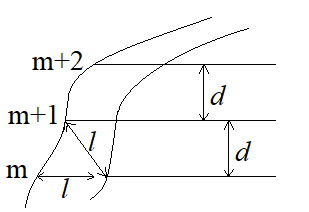
\includegraphics[width=0.7\textwidth]{obrazy/wklady_od_przekrojow.png}
\end{figure}

Pojedynczy krok ewolucji trójwymiarowej warstwy realizowany jest przez funkcję \texttt{make\_new\_layer\_3D}. Funkcja ta przyjmuje następujące argumenty:
\begin{description}
\item[\texttt{old\_layer}] \hfill \\
lista obiektów klasy \texttt{MultiPolygon} --- przekroje warstwy, która ma być ewoluowana
\item[\texttt{layer\_width}] \hfill \\
głębokość narastania warstwy w jednym kroku
\item[\texttt{l\_distance}] \hfill \\
odległość między dwoma sąsiadującymi przekrojami
\end{description}
Funkcja ta zwraca obiekt \texttt{new\_layer} --- listę przekrojów nowej warstwy. Każdy z tych przekrojów uzyskiwany jest jako przecięcie odpowiednio przeewoluowanych sąsiednich przekrojów przy użyciu metody \texttt{intersection}, która zwraca przecięcie obiektu klasy \texttt{MultiPolygon} z innym obiektem tej klasy przekazywanym jako argument. Na bazie tej funkcji stworzona została funkcja\\
\texttt{make\_N\_layers\_3D}, która poprzez wielokrotne wywołanie funkcji \texttt{new\_layer} tworzy $N$ nowych warstw. Funkcja ta zwraca listę utworzonych warstw. Do wizualizacji wzrostu agatów służy funkcja \texttt{draw\_crossection}, która rysuje przekrój o zadanym numerze agatu przekazywanego do funkcji jako lista warstw.
\section{Interferjs użytkownika}
\subsection{Część 2D}
Okno programu przedstawione jest na rysunku \ref{okno_programu_2d}.
\begin{figure}[H]
\caption{Okno programu - wersja 2D}
\label{okno_programu_2d}
\centering
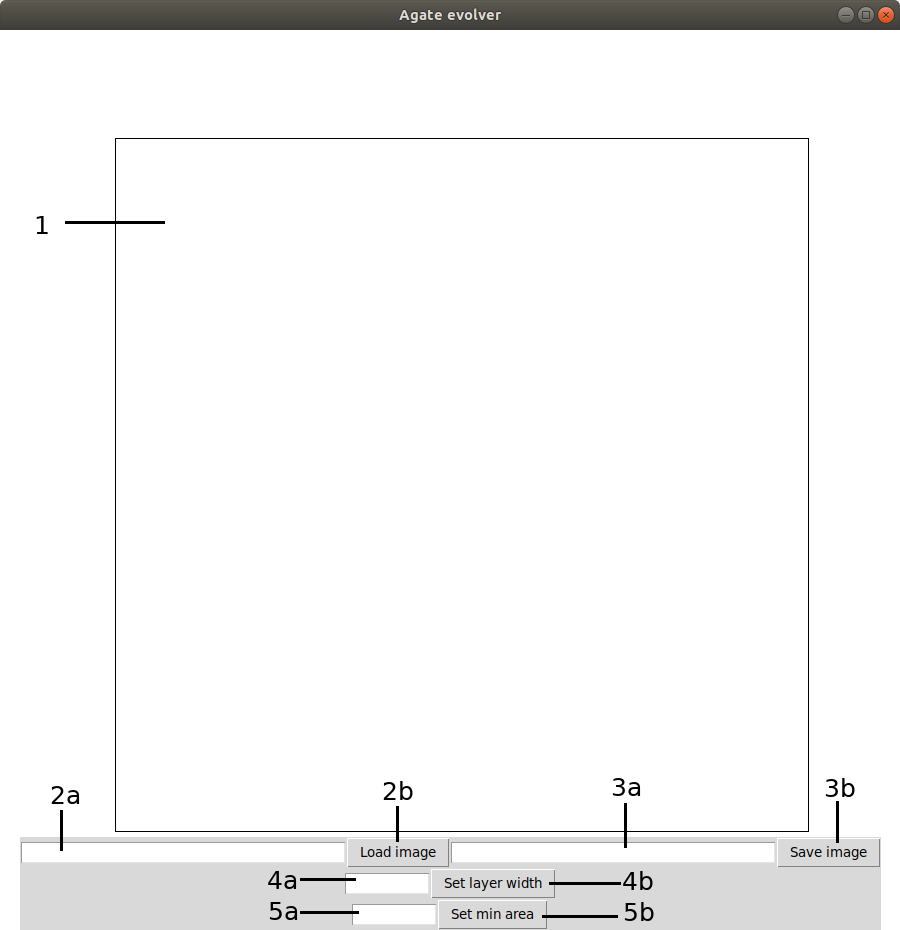
\includegraphics[width=0.75\textwidth]{obrazy/okno_programu_2d.png}
\end{figure}
Składa się z następujących części:
\begin{description}
\item[1. Obszar rysowania] \hfill \\
Użytkownik może zaznaczyć kontur agatu przytrzymując lewy przycisk myszy. W momencie puszczenia przycisku zostanie wygenerowany agat o zaznaczonym konturze. Gdy użytkownik zaczyna rysować nowy kontur, poprzedni rysunek jest usuwany. Przykład wygenerowanego agatu znajduje się na rysunku \ref{wygenerowany_agat}.
\begin{figure}[H]
\caption{Wygenerowany agat}
\label{wygenerowany_agat}
\centering
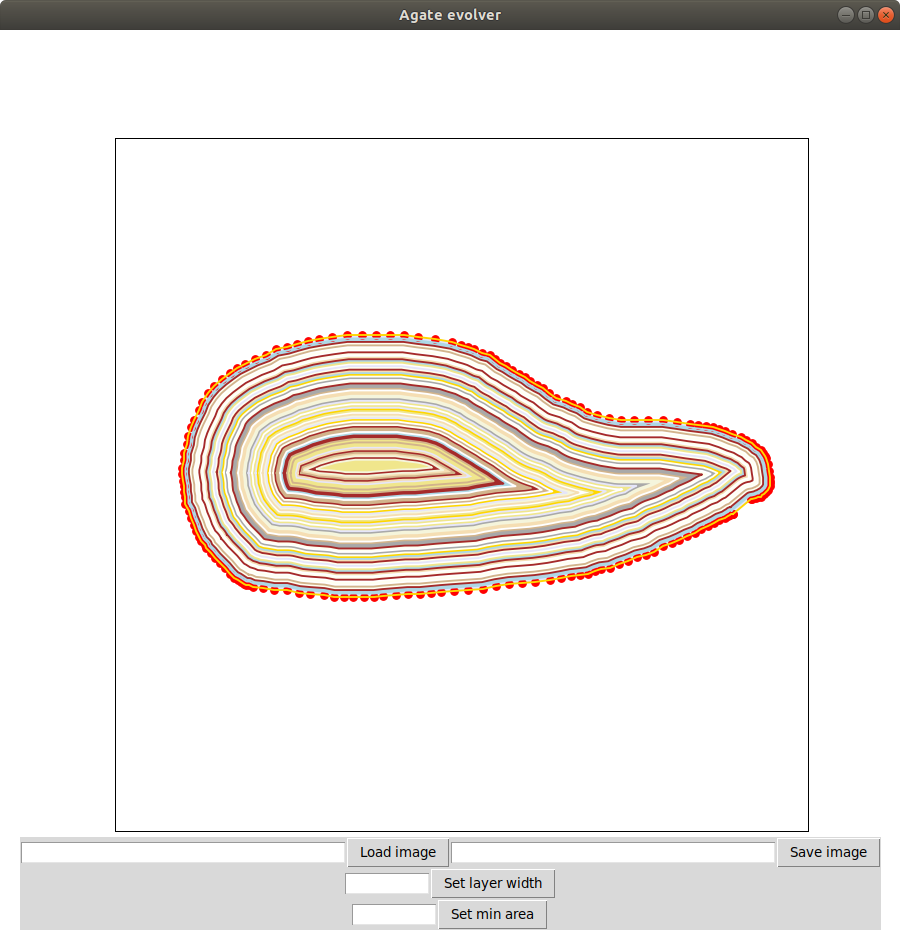
\includegraphics[width=0.75\textwidth]{obrazy/wygenerowany_agat.png}
\end{figure}
\item[2. Wczytywanie obrazu] \hfill \\
Program umożliwia wczytanie obrazu w celu porównania wyników modelu z prawdziwymi agatami. Należy podać w polu \textbf{2a} ścieżkę do pliku z obrazem w formacie PNG (można pominąć rozszerzenie), a następnie nacisnąć przycisk \textbf{2b}. Obraz zostanie wyświetlony w obszarze rysowania. Następnie można zaznaczyć w dowolnym miejscu kontur, a wygenerowany agat zostanie wyświetlony na wczytanym obrazie. Przykład takiego użycia znajduje się na rysunku \ref{agat_wygenerowany_na_rysunku}.
\begin{figure}[H]
\caption{Agat wygenerowany na rysunku}
\label{agat_wygenerowany_na_rysunku}
\centering
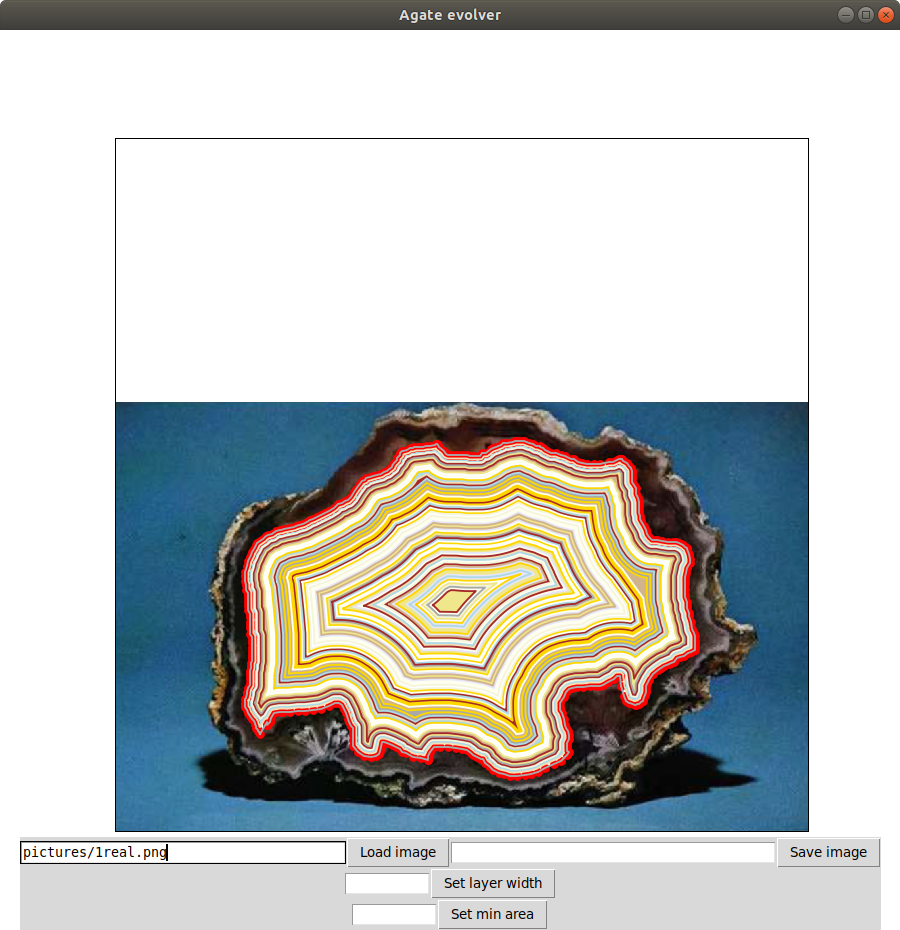
\includegraphics[width=0.75\textwidth]{obrazy/agat_wygenerowany_na_rysunku.png}
\end{figure}
\item[3. Zapisywanie obrazu] \hfill \\
Wygenerowany agat można zapisać jako obraz PNG. W tym celu należy podać w polu \textbf{3a} nazwę wynikowego pliku, a następnie nacisnąć przycisk \textbf{3b}.
\item[4. Grubość warstwy] \hfill \\
Użytkownik może ustawić grubość warstwy generowanego agatu, wpisując wartość w polu \textbf{4a}, a następnie naciskając przycisk \textbf{4b} (dla odniesienia obszar rysowania ma wymiary 1x1). Domyślna wartość: $0.005$. Przykład dwóch różnych grubości znajduje się na rysunku \ref{rozne_grubosci_warstwy}.
\begin{figure}[H]
\caption{Różne grubości warstwy}
\label{rozne_grubosci_warstwy}
\centering
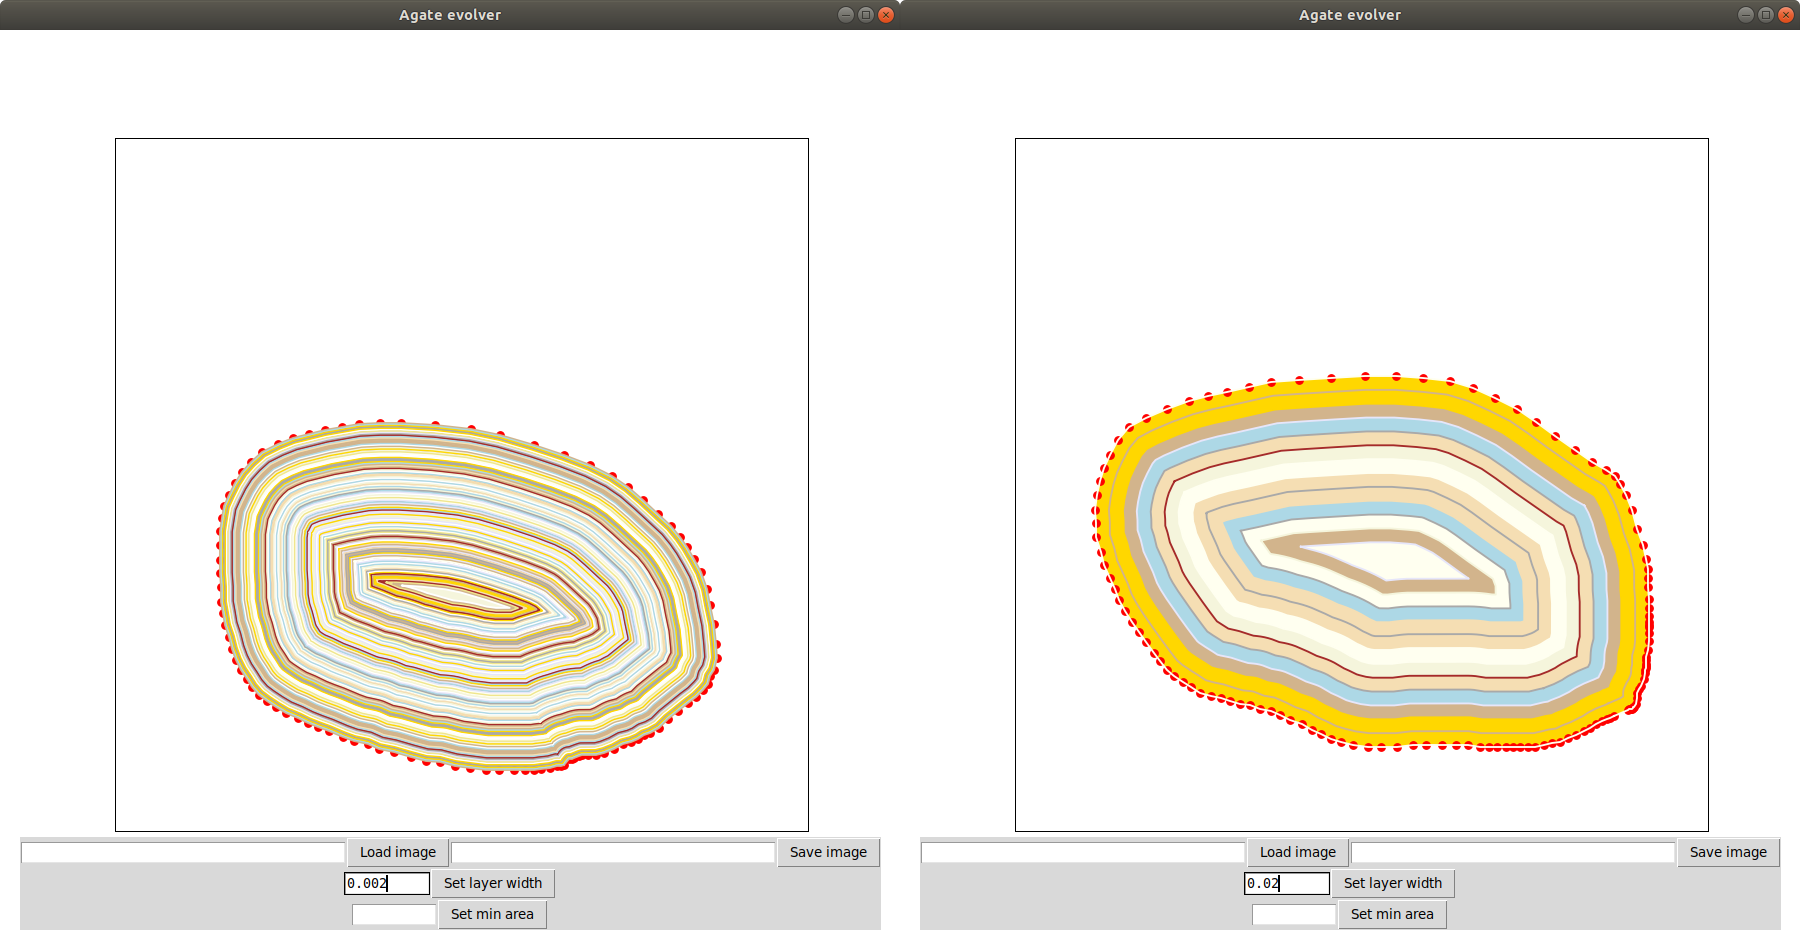
\includegraphics[width=0.75\textwidth]{obrazy/rozne_grubosci_warstwy.png}
\end{figure}
\item[5. Powierzchnia wewnętrzna] \hfill \\
Użytkownik może ustawić minimalną powierzchnię, dla której będą generowane warstwy, wpisując wartość w polu \textbf{5a}, a następnie naciskając przycisk \textbf{5b} (dla odniesienia obszar rysowania ma wymiary 1x1). Domyślna wartość: $0.001$. Parametr ten określa jak duża powinna być jednolita powierzchnia w środku generowanego agatu. Przykład dwóch różnych powierzchni znajduje się na rysunku \ref{rozne_powierzchnie_wewnetrzne}.
\begin{figure}[H]
\caption{Różne powierzchnie wewnętrzne}
\label{rozne_powierzchnie_wewnetrzne}
\centering
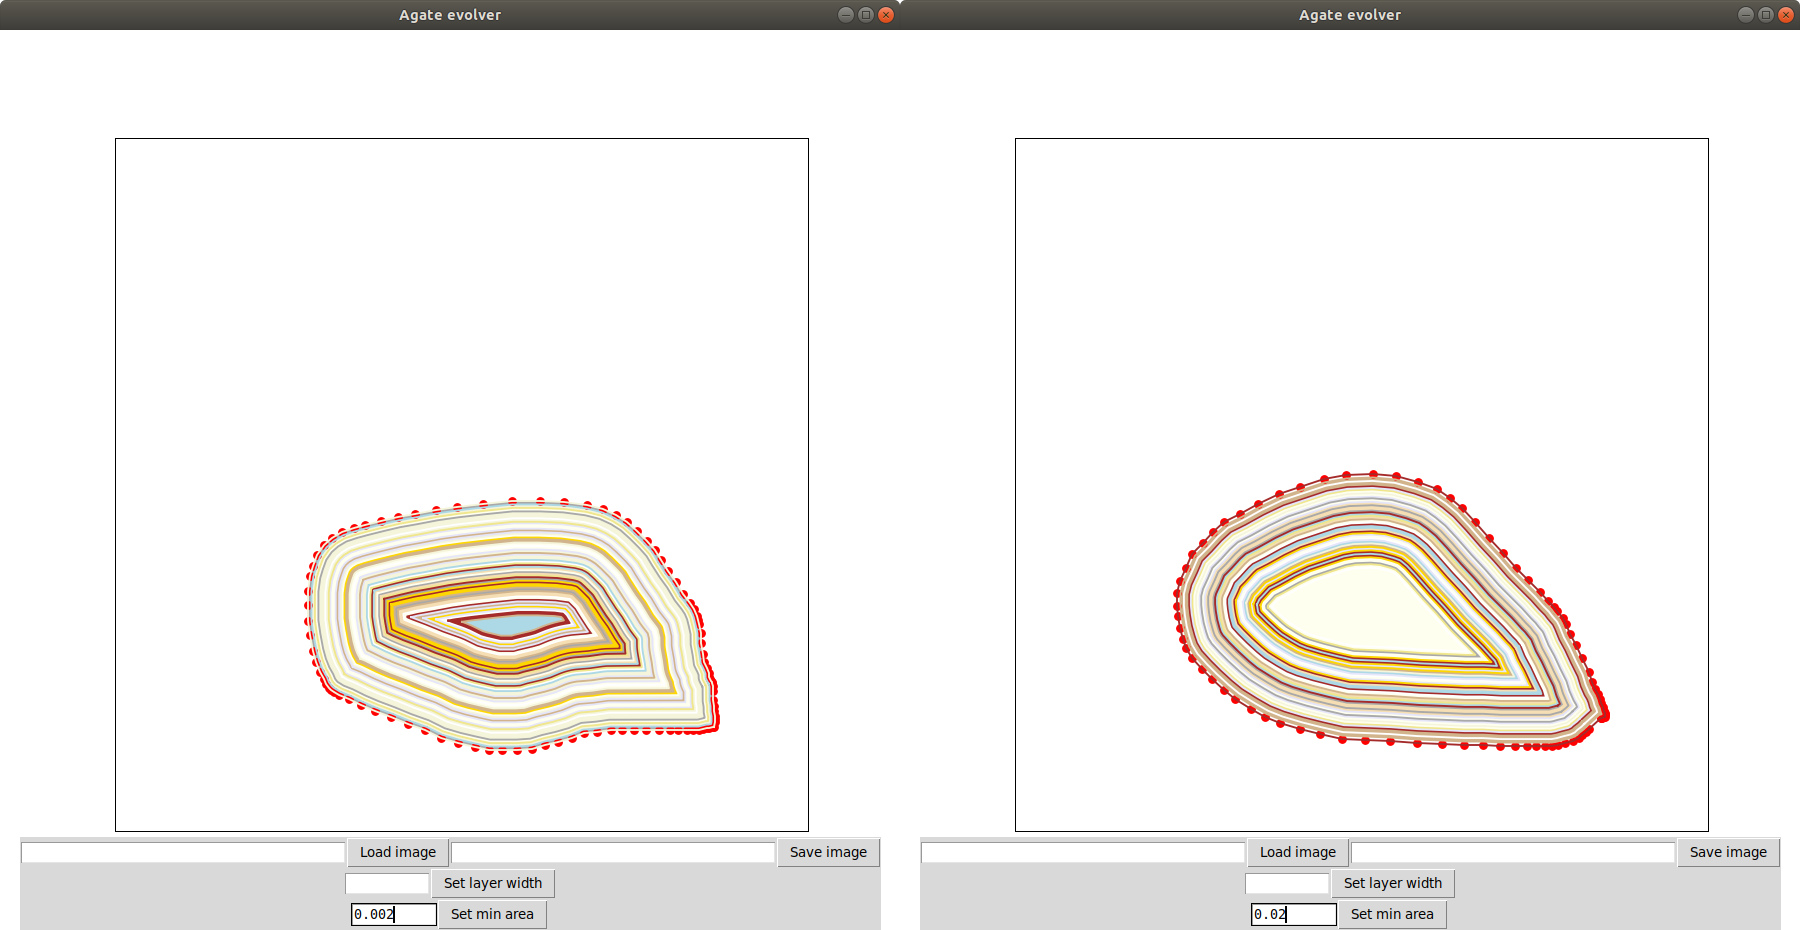
\includegraphics[width=0.75\textwidth]{obrazy/rozne_powierzchnie_wewnetrzne.png}
\end{figure}
\end{description}
\subsection{Część 3D}
Okno programu jest przedstawione na rysunku \ref{okno_programu_3d}.
\begin{figure}[H]
\caption{Okno programu - wersja 3D}
\label{okno_programu_3d}
\centering
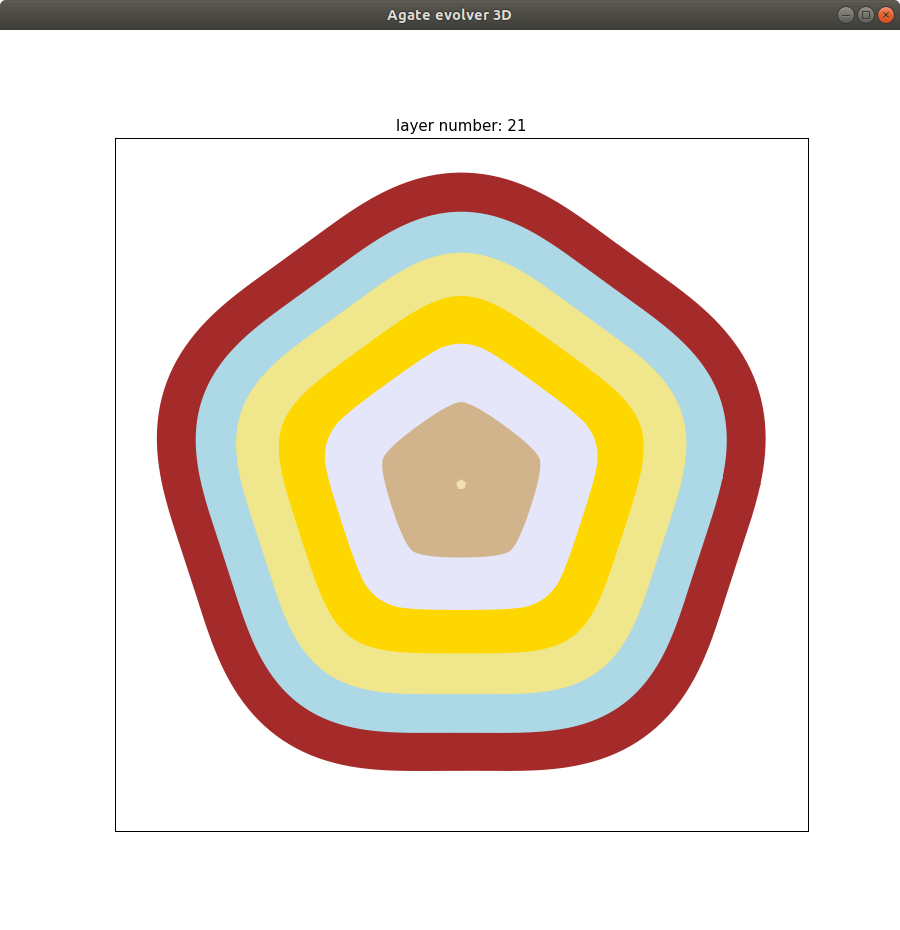
\includegraphics[width=0.75\textwidth]{obrazy/okno_programu_3d.png}
\end{figure}
Zmieniać wyświetlaną warstwę można za pomocą kółka myszy.

\section{Podsumowanie}
Mimo bardzo prostych założeń, warstwy wygenerowane w modelu 2D na podstawie konturów przekrojów prawdziwych agatów wyglądają realistycznie i w wielu przypadkach są bardzo podobne do rzeczywistych, co widać na rysunkach \ref{comparison1}, \ref{comparison2}, \ref{comparison3}, \ref{comparison4} i \ref{comparison5}. W sytuacjach, w których przewidywania modelu odbiegają od budowy agatu, różnice mogą mieć dwie główne przyczyny:
\begin{itemize}
\item Przekrój wykonano w pobliżu brzegu agatu, przez co warstwy narastające na nim spowodowały zmiany nieobejmowane przez model 2D
\item Przestrzeń, którą agat wypełniał podczas powstawania, nie miała postaci pustej bańki, lecz zawierała wewnątrz dodatkowe struktury, a jej przekrój nie był jednospójny, przez co warstwy narastały jednocześnie z wielu stron
\end{itemize}
\begin{figure}[H]
\caption{Porównanie agatu rzeczywistego i wygenerowanego}
\label{comparison1}
\centering
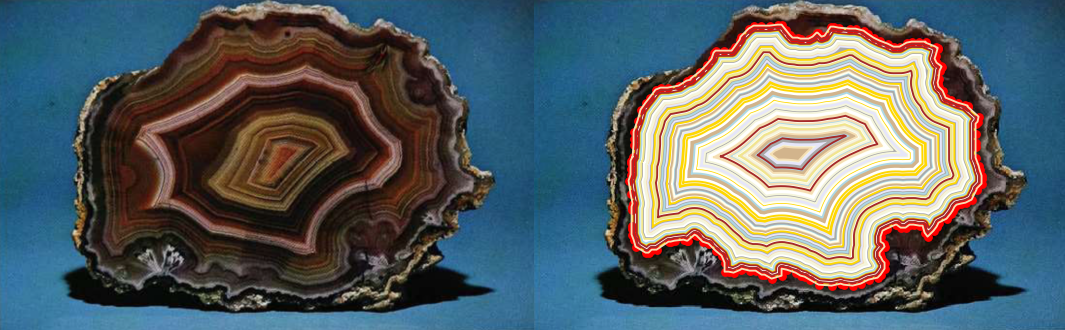
\includegraphics[width=0.75\textwidth]{obrazy/comparison/1.png}
\end{figure}
\begin{figure}[H]
\caption{Porównanie agatu rzeczywistego i wygenerowanego}
\label{comparison2}
\centering
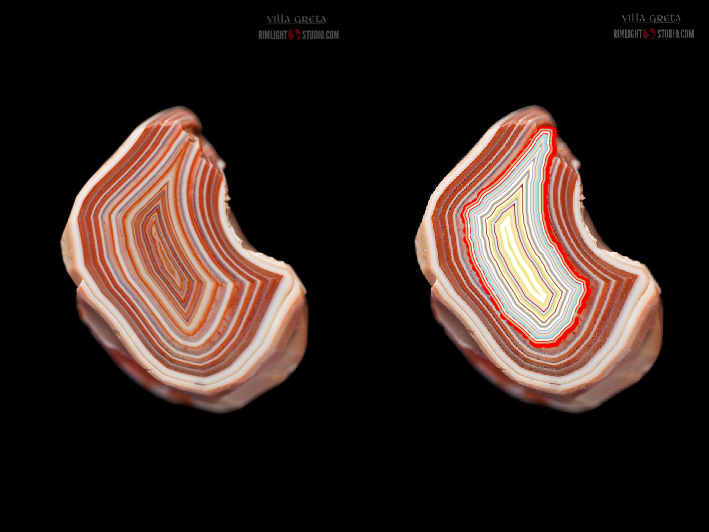
\includegraphics[width=0.75\textwidth]{obrazy/comparison/2.png}
\end{figure}
\begin{figure}[H]
\caption{Porównanie agatu rzeczywistego i wygenerowanego}
\label{comparison3}
\centering
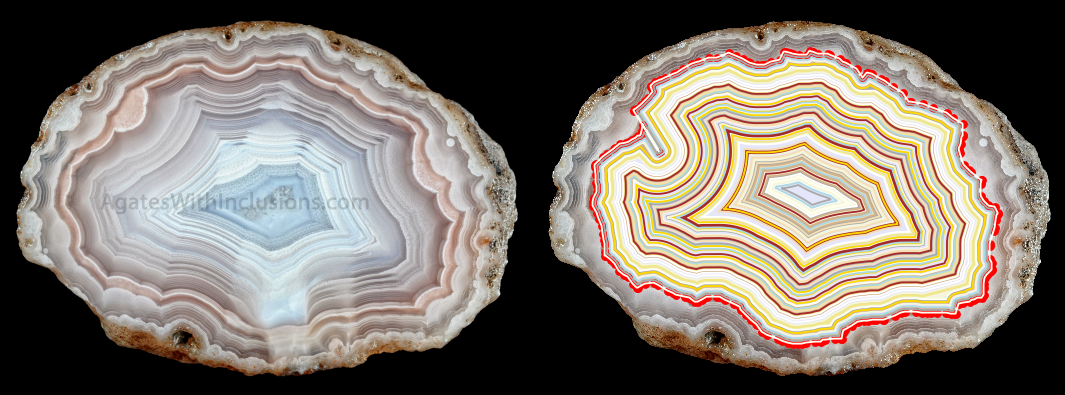
\includegraphics[width=0.75\textwidth]{obrazy/comparison/3.png}
\end{figure}
\begin{figure}[H]
\caption{Porównanie agatu rzeczywistego i wygenerowanego}
\label{comparison4}
\centering
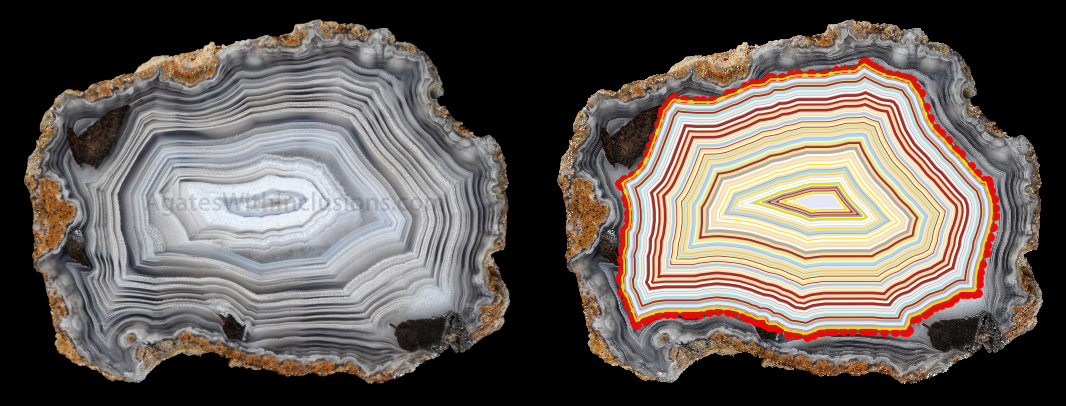
\includegraphics[width=0.75\textwidth]{obrazy/comparison/4.png}
\end{figure}
\begin{figure}[H]
\caption{Porównanie agatu rzeczywistego i wygenerowanego}
\label{comparison5}
\centering
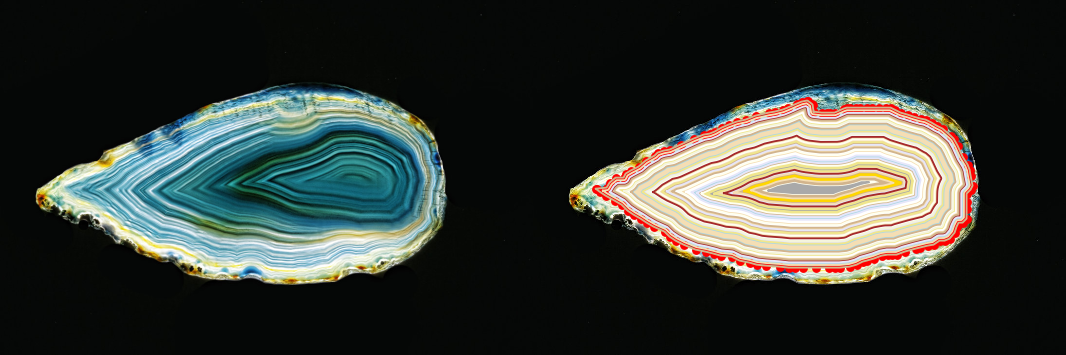
\includegraphics[width=0.75\textwidth]{obrazy/comparison/5.png}
\end{figure}
\end{document}

